%%%%%%%%%%%%%%%%%%%%%%%%%%%%%%%%%%%%%%%%%%%%%%%%%%%%%%%%%%%%%%%%%%%%%%%%%%%%%
% Chapter 1: Introducci�n 
%%%%%%%%%%%%%%%%%%%%%%%%%%%%%%%%%%%%%%%%%%%%%%%%%%%%%%%%%%%%%%%%%%%%%%%%%%%%%%%

%---------------------------------------------------------------------------------
\section{Antecedentes y estado actual del tema}
\label{1:sec:1}

La \ceit{World Wide Web} esta sujeta a un cambio continuo. La llegada de \ceit{HTML5}, la creciente importancia de \ceit{AJAX} y de la 
programaci\'on en el lado del cliente, las nuevas fronteras de la \ceit{Web Sem\'antica}, la explosi\'on de las redes 
sociales as\'{\i} como la llegada de las redes sociales federadas son ejemplos de esta tendencia general. 
Las aplicaciones web parecen evolucionar hacia entornos cada vez m\'as ricos y flexibles en los que los usuarios 
pueden acceder con facilidad a los documentos, publicar contenido, escuchar m\'usica, ver v\'{\i}deos, realizar dibujos
e incluso jugar usando un navegador. Esta nueva clase de software ubicuo no cesa de ganar \textit{momentum} y promueve nuevas 
formas de interacci\'on y cooperaci\'on.
\bigskip

Dentro del \'ambito educativo tambi\'en se ha vivido una revoluci\'on, en forma y contenido, de impartir ense�anza.
En Internet se puede encontrar, cada vez con m\'as facilidad, contenidos de cualquier disciplina en m\'ultiples
formatos: blogs, videotutoriales, presentaciones, ejercicios resueltos, etc.

Tambi\'en est\'an teniendo mucho \'exito las plataformas de aprendizaje virtual ofreciendo, adem\'as de conocimiento 
sin la necesidad de estar f\'{\i}sicamente presente en un aula, una serie de recompensas y medallas por ir obteniendo
logros. Esta metodolog\'{\i}a se denomina \ceis{Gamificaci\'on} y est\'a teniendo un impacto muy positivo en los usuarios
de estas plataformas, ya que los anima a seguir usando estas herramientas de conocimiento.
\bigskip

Otro tipo de plataforma de aprendizaje virtual m\'as orientada a universidades e institutos es \ceis{Moodle}. Est\'a implamantada
en numerosos centros de todo el planeta. Es el complemento perfecto para enriquecer las ense�anzas impartidas f\'{\i}sicamente
con cuestionarios autoevaluativos y compartici\'on de recursos adicionales. Adem\'as, facilita numerosas tareas a los docentes como 
la correcci\'on y calificaci\'on de ejercicios.

Sin embargo, esta plataforma s\'olo se limita a la evaluaci\'on de cuestiones triviales. Para la correci\'on de preguntas
propias de las ramas de \ceit{Ingenier\'{\i}a}, como pueden ser la implementaci\'on de c\'odigo, es necesaria la figura del profesor para
evaluar dichas tareas.

Otro problema que presenta es su dif\'{\i}cil portabilidad. Estamos hablando de un tipo de plataforma que sigue un
esquema \ceis{cliente-servidor}, que no es f\'acilmente migrable a otras m\'aquinas.
\bigskip

%XXXX  a�adir las ventajas del nuevo ruql comparativamente

% \section{Usuario al que va Destinado Ruql}

Estas desventajas se ven resueltas, haciendo uso de \ceis{RuQL}, en la {\bfseries Aplicaci\'on para la Elaboraci\'on y Despliegue de Cuestionarios} que se presentar\'a
en esta memoria. Dicha aplicaci\'on est\'a destinada a profesores con ciertos conocimientos en el \'ambito de la programaci\'on y de la inform\'atica, 
aunque la curva de aprendizaje no es excesiva para el resto del profesorado.

%---------------------------------------------------------------------------------
\section{�Qu\'e es \ceit{RuQL}?}
\label{1:sec:2}

Esta aplicaci\'on de generaci\'on y despliegue de cuestionarios hace uso de una
gema de Ruby creada por \href{http://www.armandofox.com/geek}{Armando Fox} denominada 
\href{http://github.com/saasbook/ruql}{'Ruby-based Quiz Generator and DSL'} (RuQL).
%XXXXXX expandir como fu� el proceso de contacto con Armando

Inicialmente, esta gema permit\'{\i}a generar un cuestionario partiendo de un fichero \ceis{Ruby}, 
donde se redactaban las preguntas y respuestas haciendo uso de un \ceis{DSL}.

Pose\'{\i}a una serie de \textit{renderers} que permit\'{\i}an generar los cuestionario en los siguientes formatos:
\begin{itemize}
  \item \href{http://code.edx.org/}{\ceit{Open EdX}}: formato \cei{open source} listo para importar en plataformas de aprendizaje online como \ceis{EdX}.
  \item Versi\'on \ceit{HTML5} imprimible: lista para ser impresa y rellenada por los usuarios.
  Se le pod\'{\i}a pasar como argumento el path de una hoja de estilo para incorporarla al \ceit{HTML} de salida. Del mismo modo, se
  pod\'{\i}a especificar el path de un template predefinido por el profesor de modo que las preguntas se renderizaran en el mismo.
  \item \href{http://home.gna.org/auto-qcm}{\ceit{AutoQCM}}: formato listo para importar a \ceis{AMC} (\textit{Auto Multiple Choice}), software libre
  que permite elaborar cuestionarios multirrespuesta.
\end{itemize}
\bigskip

Los tipos de preguntas que se pod\'{\i}an especificar eran:
\begin{itemize}
  \item {\bfseries Preguntas de completar}: en las cuales los usuarios deben rellenar los espacios en blanco. Admit\'{\i}a respuestas de tipo \cei{string} o
  \cei{regexp}. Si exist\'{\i}an m\'ultiples espacios para rellenar, se especificaban las respuestas en forma de \cei{array}, indicando adem\'as
  si el orden de las mismas influ\'{\i}a.
  Permit\'{\i}a adem\'as especificar respuestas falsas (\textit{distractors}) con una explicaci\'on de la misma, de modo que si el 
  alumno escrib\'{\i}a dicho \cei{distractor}, le apareciera la explicaci\'on de por qu\'e esa respuesta era incorrecta.
  
  \begin{figure}[!th]
  \begin{center}
  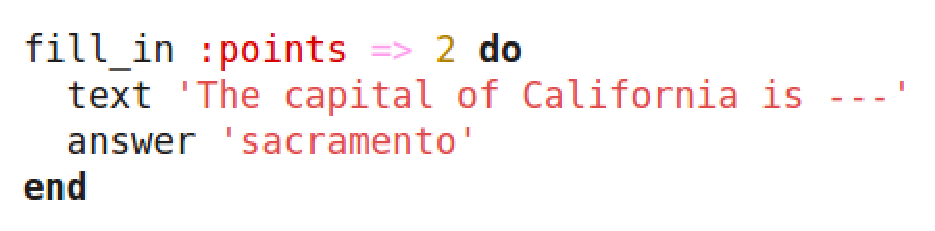
\includegraphics[width=0.6\textwidth]{images/fill_in1.eps}
  \caption{Pregunta de completar simple}
  \label{fig:fill_in1}
  \end{center}
  \end{figure}
  
  \begin{figure}[!th]
  \begin{center}
  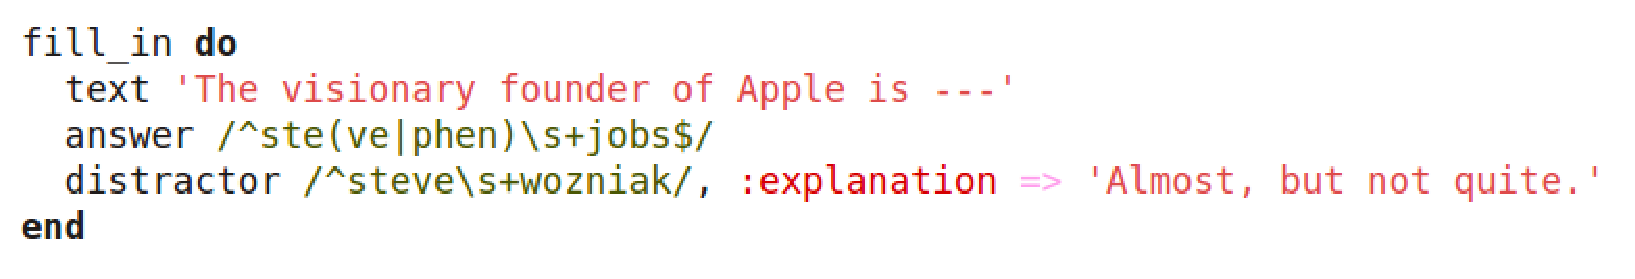
\includegraphics[width=1\textwidth]{images/fill_in2.eps}
  \caption{Pregunta de completar con distractor y explicaci\'on}
  \label{fig:fill_in2}
  \end{center}
  \end{figure}
  
  \item {\bfseries Preguntas multirrespuesta con una  \'unica respuesta correcta}: las cl\'asicas preguntas tipo test. Se pod\'{\i}a aleatorizar el orden
  de las respuestas definido en el fichero de preguntas y asignarles explicaciones a los \textit{distractors} de manera individual o asignar una explicaci\'on
  general para todos los \textit{distractors}.
  \bigskip
  
  \begin{figure}[!th]
  \begin{center}
  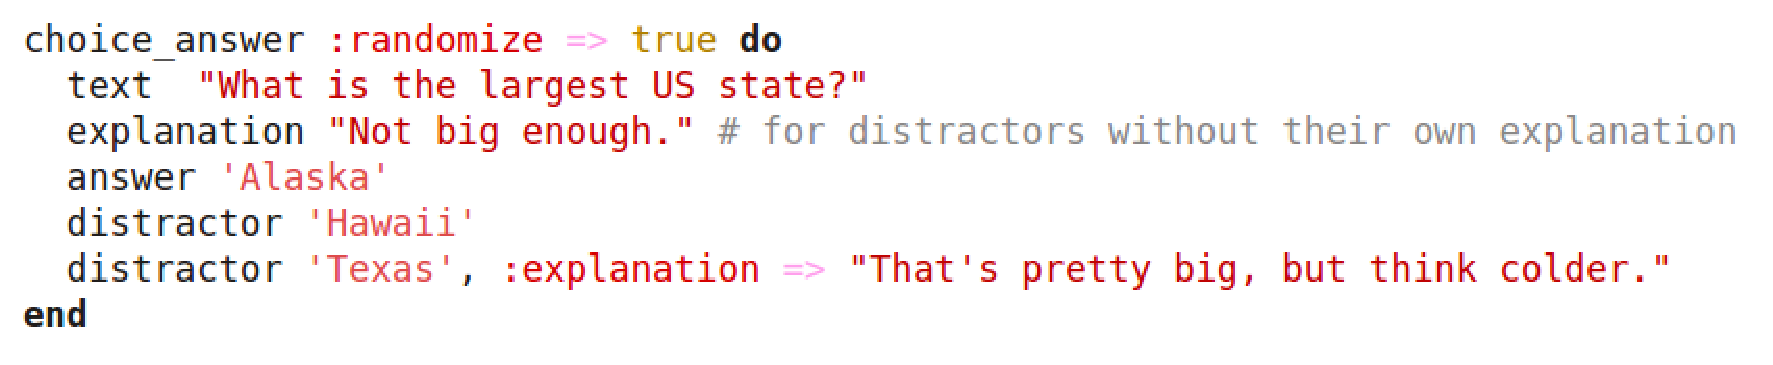
\includegraphics[width=1\textwidth]{images/choice_answer1.eps}
  \caption{Pregunta multirrespuesta con una  \'unica respuesta correcta}
  \label{fig:choice_answer1}
  \end{center}
  \end{figure}
  
  Especificando adem\'as la opci\'on \cei{raw} a la pregunta, permit\'{\i}a incrustar dicho texto entre etiquetas \textless pre\textgreater \space \ceit{HTML}.
 
  \begin{figure}[H]
  \begin{center}
  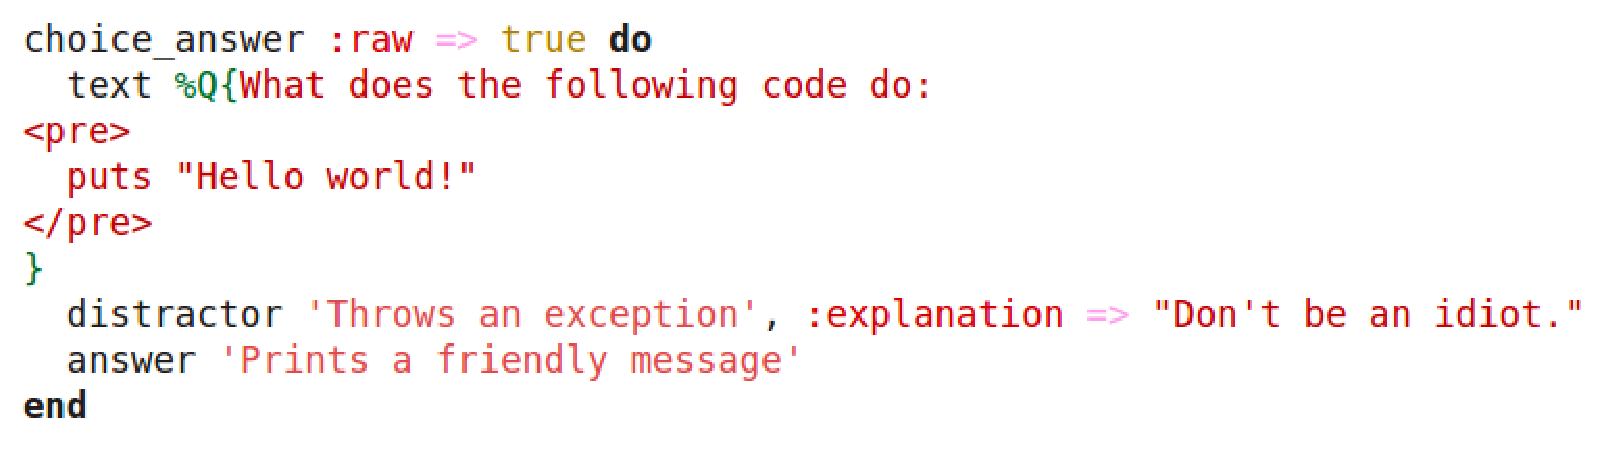
\includegraphics[width=0.9\textwidth]{images/choice_answer2.eps}
  \caption{Pregunta multirrespuesta usando la opci\'on \textit{raw}}
  \label{fig:choice_answer2}
  \end{center}
  \end{figure}
  
  \item {\bfseries Preguntas multirrespuesta con una  m\'ultiples respuestas correctas}: iguales a las preguntas multirrespuesta de opci\'on \'unica con la diferencia de 
  que existe m\'as de una respuesta correcta.
 
  \begin{figure}[H]
  \begin{center}
  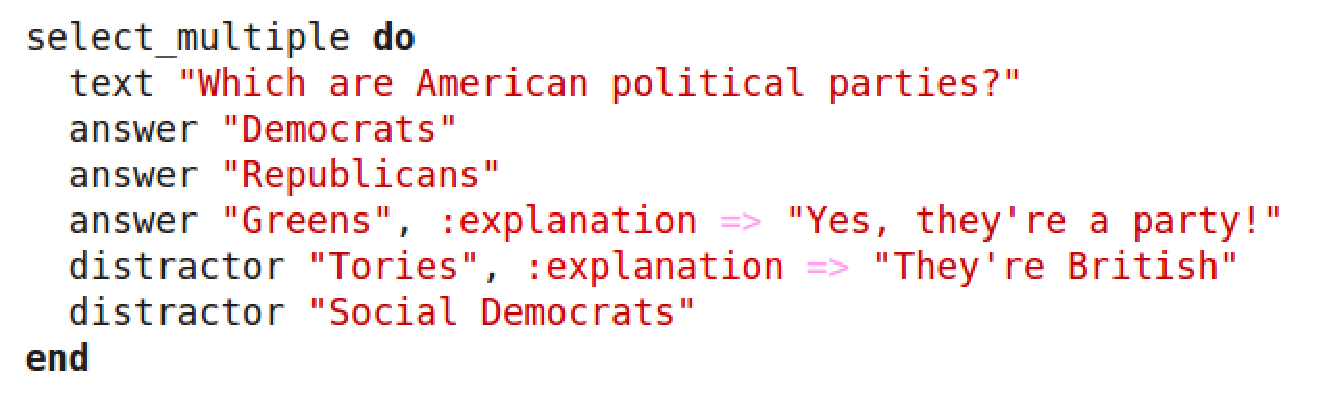
\includegraphics[width=0.8\textwidth]{images/select_multiple.eps}
  \caption{Pregunta multirrespuesta con una  m\'ultiples respuestas correctas}
  \label{fig:select_multiple}
  \end{center}
  \end{figure}
  
  \item {\bfseries Preguntas de verdadero o falso}: caso particular de las preguntas multirrespuesta de opci\'on \'unica.
  
  \begin{figure}[!th]
  \begin{center}
  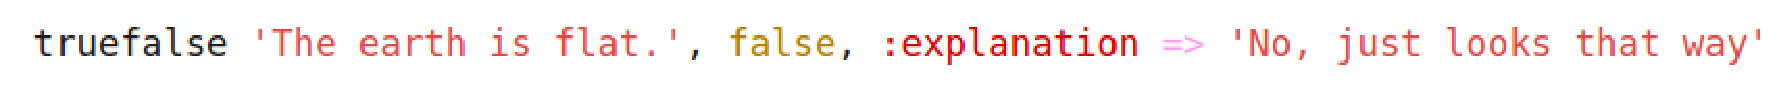
\includegraphics[width=1\textwidth]{images/truefalse.eps}
  \caption{Pregunta de verdadero o falso}
  \label{fig:truefalse}
  \end{center}
  \end{figure}
  
\end{itemize}

Para todos los tipos de preguntas era posible especificar un comentario opcional que acompa�ar\'{\i}a al texto de la pregunta.
\bigskip

\subsection{C\'odigo de ejemplo para realizar un cuestionario HTML5}
\label{subsec:1.2.1}
Instalamos la gema:

\begin{verbatim}
[~]$ gem install ruql
Fetching: ruql-0.0.4.gem (100%)
Successfully installed ruql-0.0.4
1 gem installed
\end{verbatim}

Creamos el fichero Ruby que contendr\'a las preguntas:

\begin{verbatim}
[~]$ cd tmp
[~/tmp]$ mkdir example
[~/tmp]$ vi example.rb
[~/tmp]$ cat example.rb 
\end{verbatim}

\begin{lstlisting}
quiz 'Example quiz' do
  
  fill_in :points => 2 do
    text 'The capital of California is ---'
    answer 'sacramento'
  end
  
  choice_answer :randomize => true do
    text  "What is the largest US state?"
    explanation "Not big enough." # for distractors without their own explanation
    answer 'Alaska'
    distractor 'Hawaii'
    distractor 'Texas', :explanation => "That's pretty big, but think colder."
  end
  
  select_multiple do
    text "Which are American political parties?"
    answer "Democrats"
    answer "Republicans"
    answer "Greens", :explanation => "Yes, they're a party!"
    distractor "Tories", :explanation => "They're British"
    distractor "Social Democrats"
  end
  
  select_multiple do
    text "Which are American political parties?"
    answer "Democrats"
    answer "Republicans"
    answer "Greens", :explanation => "Yes, they're a party!"
    distractor "Tories", :explanation => "They're British"
    distractor "Social Democrats"
  end
  
  truefalse 'The week has 7 days.', true
  truefalse 'The earth is flat.', false, :explanation => 'No, just looks that way'
\end{lstlisting}
\bigskip

Para generar el HTML versi\'on imprimible, ejecutamos el siguiente comando:

\begin{verbatim}
[~/tmp]$ ruql example.rb Html5 > example.html
\end{verbatim}

Si deseamos que nuestras preguntas se rendericen usando nuestro propio template, debemos especificarlo con la opci\'on -t:

\begin{verbatim}
[~/tmp]$ ruql example.rb Html5 -t template.html.erb > example.html
\end{verbatim}

Las especificaciones de c\'omo crear nuestro propio template se encuentran en el apartado de Gu\'{\i}a de usuario (v\'ease Ap\'endice \ref{Apendice2}).

%---------------------------------------------------------------------------------
\section{Objetivos y actividades a realizar}
\label{1:sec:3}

Los objetivos propuestos para alcanzar en este Trabajo de Fin de Grado ha sido los siguientes:
\begin{itemize}
  \item Conocer, dominar y practicar con lenguajes y herramientas de desarrollo de aplicaciones web en el \ceis{servidor}.
  \item Conocer, dominar y practicar con diferentes lenguajes y librer\'{\i}as en el \ceis{cliente}.
  \item Conocer, practicar y dominar de herramientas de \ceis{desarrollo dirigido por pruebas} (\textit{TDD}) en entornos web.
  \item Conocer, practicar y dominar diferentes lenguajes de marcas y de estilo.
  \item Conocer, practicar y dominar diferentes mecanismos de despliegue.
  \item Conocer, practicar y familiarizarse con diferentes mecanismos de \ceit{seguridad}, \ceit{autentificaci\'on} y \ceit{autorizaci\'on}.
  \item Conocer, practicar y dominar diferentes herramientas colaborativas y de \ceis{control de versiones} (\textit{CVS}).
  \item Conocer, practicar y dominar \ceis{metodolog\'{\i}as \'agiles} de desarrollo de software.
  \item Desarrollar una aplicaci\'on web para la elaboraci\'on y \ceit{despliegue} de cuestionarios.
\end{itemize}
\bigskip

Y las actividades a realizar en el mismo, tal cual est\'an descritas en la propuesta de {\bfseries Proyecto de Trabajo de Fin de Grado} firmada por 
el director y el alumno en la actividad 2 de la asignatura, son las que se describen a continuaci\'on:
\begin{itemize}
  \item Revisi\'on bibliogr\'afica.
  \item Realizaci\'on de una \ceit{aplicaci\'on web} en la que:
  \begin{itemize}
    \item Se proporciona soporte mediante una aplicaci\'on web a los procesos de evaluaci\'on.
    \item Se proporciona/extiende un \ceis{Lenguaje de Dominio Espec\'{\i}fico} (\textit{DSL}) para la elaboraci\'on de cuestionarios.
    \item Se deber\'a considerar c\'omo resolver los problemas de \ceit{seguridad} asociados.
    \item Redacci\'on de la memoria.
  \end{itemize}
  \item Preparaci\'on de las presentaciones.
\end{itemize}



%---------------------------------------------------------------------------------
\section{Tecnolog\'{\i}a usada}
\label{1:sec:4}

Debido a que este Trabajo de Fin de Grado es una extensi\'on de una \ceit{gema} de \ceis{Ruby}, se ha utilizado \'este como \ceit{lenguaje de
programaci\'on}.

\begin{center}

\includegraphics{images/ruby.eps}
\end{center}
  
Adem\'as, se ha hecho uso de un numeroso conjunto de gemas y de otras tecnolog\'{\i}as enumeradas a continuaci\'on:
\begin{itemize}
  \item \ceit{HTML5}        
\includegraphics[width=0.13\textwidth]{images/HTML5.eps}
  \item \ceit{CSS3}         
\includegraphics[width=0.1\textwidth]{images/css3.eps}
  \item \ceit{JavaScript}   
\includegraphics[width=0.1\textwidth]{images/js.eps}
  \item \ceit{Bootstrap}    
\includegraphics[width=0.1\textwidth]{images/bootstrap.eps}
  \item \ceit{jQuery}       
\includegraphics[width=0.2\textwidth]{images/jquery.eps}
  \item \ceit{XRegExp}      
\includegraphics[width=0.2\textwidth]{images/xregexp.eps}
  \item \ceit{MathJax}      
\includegraphics[width=0.2\textwidth]{images/mathjax.eps}
  \item \ceit{CodeMirror}   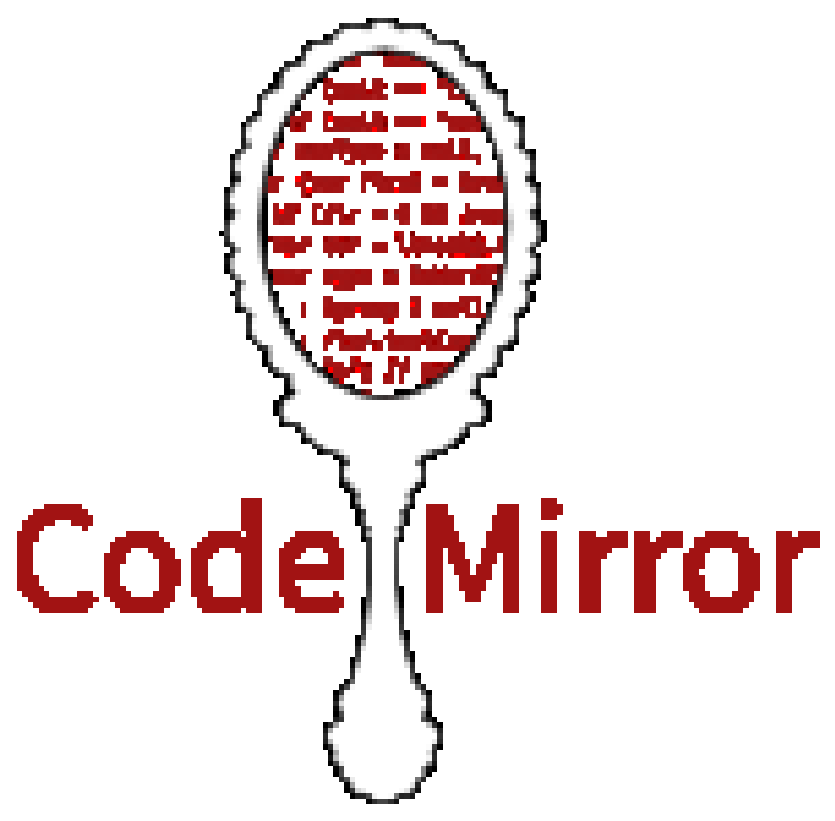
\includegraphics[width=0.1\textwidth]{images/codemirror.eps}
  \item \ceit{Mocha}        
\includegraphics[width=0.1\textwidth]{images/mocha.eps}
  \item \ceit{Chai}         
\includegraphics[width=0.1\textwidth]{images/chai.eps}
  \item \ceit{Karma}        
\includegraphics[width=0.1\textwidth]{images/karma.eps}
  \item \ceit{Sinatra}      
\includegraphics[width=0.1\textwidth]{images/sinatra.eps}
  \item \ceit{GitHub}       
\includegraphics[width=0.1\textwidth]{images/github.eps}
  \item \ceit{Heroku}       
\includegraphics[width=0.1\textwidth]{images/heroku.eps}
  \item \ceit{OAuth 2.0}    
\includegraphics[width=0.1\textwidth]{images/oauth.eps}
  \item \ceit{Google Drive} 
\includegraphics[width=0.1\textwidth]{images/google_drive.eps}
\end{itemize}

